\documentclass{sigchi}

% Use this command to override the default ACM copyright statement (e.g. for preprints). 
% Consult the conference website for the camera-ready copyright statement.


%% EXAMPLE BEGIN -- HOW TO OVERRIDE THE DEFAULT COPYRIGHT STRIP -- (July 22, 2013 - Paul Baumann)
% \toappear{Permission to make digital or hard copies of all or part of this work for personal or classroom use is 	granted without fee provided that copies are not made or distributed for profit or commercial advantage and that copies bear this notice and the full citation on the first page. Copyrights for components of this work owned by others than ACM must be honored. Abstracting with credit is permitted. To copy otherwise, or republish, to post on servers or to redistribute to lists, requires prior specific permission and/or a fee. Request permissions from permissions@acm.org. \\
% {\emph{CHI'14}}, April 26--May 1, 2014, Toronto, Canada. \\
% Copyright \copyright~2014 ACM ISBN/14/04...\$15.00. \\
% DOI string from ACM form confirmation}
%% EXAMPLE END -- HOW TO OVERRIDE THE DEFAULT COPYRIGHT STRIP -- (July 22, 2013 - Paul Baumann)


% Arabic page numbers for submission. 
% Remove this line to eliminate page numbers for the camera ready copy
\pagenumbering{arabic}


% Load basic packages
\usepackage{balance}  % to better equalize the last page
\usepackage{graphics} % for EPS, load graphicx instead
\usepackage{times}    % comment if you want LaTeX's default font
\usepackage{url}      % llt: nicely formatted URLs
\usepackage{color}

\usepackage{pdflscape}
\usepackage{longtable}
% \usepackage{geometry}
\usepackage[strict]{changepage}
\usepackage{german}


% llt: Define a global style for URLs, rather that the default one
\makeatletter
\def\url@leostyle{%
  \@ifundefined{selectfont}{\def\UrlFont{\sf}}{\def\UrlFont{\small\bf\ttfamily}}}
\makeatother
\urlstyle{leo}


% To make various LaTeX processors do the right thing with page size.
\def\pprw{210mm}
\def\pprh{297mm}
\special{papersize=\pprw,\pprh}
\setlength{\paperwidth}{\pprw}
\setlength{\paperheight}{\pprh}
\setlength{\pdfpagewidth}{\pprw}
\setlength{\pdfpageheight}{\pprh}

% Make sure hyperref comes last of your loaded packages, 
% to give it a fighting chance of not being over-written, 
% since its job is to redefine many LaTeX commands.
\usepackage[pdftex]{hyperref}
\hypersetup{
pdftitle={Supporting public deliberation through spatially enhanced dialogues},
pdfauthor={LaTeX},
bookmarksnumbered,
pdfstartview={FitH},
colorlinks,
citecolor=black,
filecolor=black,
linkcolor=black,
urlcolor=black,
breaklinks=true,
}

% create a shortcut to typeset table headings
\newcommand\tabhead[1]{\small\textbf{#1}}

% End of preamble. Here it comes the document.
\begin{document}

\title{Supporting public deliberation\\through spatially enhanced dialogues}
\subtitle{Master thesis}

\numberofauthors{1}
\author{
  \alignauthor Gerald Pape\\
    \affaddr{Institute for Geoinformatics}\\
    \email{g.pape@uni-muenster.de}\\
%   \alignauthor 2nd Author Name\\
%     \affaddr{Affiliation}\\
%     \affaddr{Address}\\
%     \email{e-mail address}\\
%     \affaddr{Optional phone number}    
%   \alignauthor 3rd Author Name\\
%     \affaddr{Affiliation}\\
%     \affaddr{Address}\\
%     \email{e-mail address}\\
%     \affaddr{Optional phone number}
}

\maketitle

\begin{abstract}
swaghetti yolonaise
\end{abstract}

% \keywords{
% 	Guides; instructions; author's kit; conference publications;
% 	keywords should be separated by a semi-colon.
% 	\textcolor{red}{Mandatory section to be included in your final version.}
% }

% \category{H.5.m.}{Information Interfaces and Presentation (e.g. HCI)}{Miscellaneous}

% See: \url{http://www.acm.org/about/class/1998/}
% for more information and the full list of ACM classifiers
% and descriptors. 
% \textcolor{red}{Mandatory section to be included in your
% final version. On the submission page only the classifiers'
% letter-number combination will need to be entered.}

\section{Introduction}
Since their first appearance, Web 2.0 applications utilized their collaborative character to gather information and opinions from their users. Today, modern information technologies are ubiquitous in many aspects of daily life. Involving citizens in decision processes around public matters through such applications has formed the field of ``eParticipation''. Its premise is to strengthen democratic processes between citizens and its governments through said modern information technologies \cite{Saebo_eParticipation, Medaglia2012_eParticipation}. One of many aspects is public deliberation which revolves around engaging citizen in dialogues about 


\section{Related Work}

\subsubsection{Argumentation mapping}
Rinner\cite{Rinner_ArgumentationMaps}\dots

Existing implementations\dots

Evaluation\dots
\subsubsection{Public deliberation and eParticipation}


\section{Approach}



\subsubsection{DialogMap}

In order to test the initial idea of supporting public deliberation through spatially enhanced dialogues, a working prototype had to be developed. Starting from an initial survey of existing research, a first prototypical application was developed. This prototype was then extended and refined with practical advice from members of a scientific citizens' initiative. Their input ranged from general suggestions to opinions of specific features. This chapter will give some details of design and implementation of the developed developed.


\subsubsection{Design decisions} % and features

As seen in X,Y and Z, important aspects of A are\dots

Internally, the prototype uses few data models. Contributions contain a title, description, two categories, a tags field, a favored counter, an optional time restriction field for start and ending times, an optional image, an optional reference to a parent contribution and optional references to child contributions. The parent and child contribution references create a simple parent-child connection between contributions, as children inherit the categories, tags, time restriction and title. A contribution serves both as a topic and as response to a topic. A contribution also contains references to features, references to features and references to URLs.\\
Features are geospatial entities with a spatial location, a reference to its contribution and properties for styling\footnote{\url{https://github.com/mapbox/simplestyle-spec}}.\\
Feature references contain a description of the featurea and the reference to a feature. URL references contain hyperlinks and a description of the hyperlink. The description of a contribution contains the text typed by a user with specially encoded references to features, URL references and feature references.\\
After signing in, users can create contributions in the manner of creating topics or writing responses to existing topics. Users have an e-mail address and a name.

The front page of the prototype puts a map side by side with a sidebar at right hand side containing from top to bottom the input form for new contributions, filter options, sorting order selector and a list of contributions. The input form consists of input fields for title, categories, time restriction, image and description. The description field allows the creation of spatial features and URL/feature references through connecting words with spatial representations or URLs.\\
A free text input field and multiple checkboxes allow to restrict the listed contribution as well as the geo-features displayed in the map. It is also possible to change the order of the list of contribution through a drop down field.\\
The list of contributions contains colored rectangles representing the different topics. Each box contains the title, time of writing, name of the author, categories, tags and the amount of times the contribution has been favored by users. It also contains a link which navigates to the replies written to the topic. A click on the contribution box expands it, revealing the description of the current topic.\\
After clicking the ``reply'' link, only the selected topic and replies are shown in the sidebar in a chronological order. In this view, each contribution shows the description by default as well as author and time and date of writing. The author of the contribution is able to edit the contribution. Other users are able to favor the contribution to show interest or agreement.\\
The map view contains a base map and several markers and polygons in different colors and different icons in case of markers. These relate to the contributions and are connected through the references in the description of the contributions. Which spatial features are displayed is determined through the state of the sidebar. In the topics overview, only the features created for the starting contribution are displayed in order to prevent cluttering of the view-port. When only the topic and its replies are displayed in the sidebar, all features related to the topic and its replies are shown on the map.\\
To emphasize the relationship between a contribution and its spatial features, a two way highlighting has been implemented. Hovering over either a contribution-box, marked word or spatial feature on the map triggers visual highlighting on all related contributions, marked words and spatial features. This allows to quickly grasp the relationship between features and contributions.\\
Users are able to use either traditional sing-up/sign-in methods or social sign-in through different providers to authenticate to the system.

% \begin{itemize}
% \item Map view with sidebar on right hand side
% \item Two way highlighting between contributions in sidebar and features on map
% \item Creation of Topic with \begin{itemize}
%     \item Title
%     \item Category/ies \begin{itemize}
%         \item in this specific case for two dimensions \begin{itemize}
%             \item Color
%             \item Icon
%             \end{itemize}
%         \end{itemize}
%     \item Tags
%     \item Time limit
%     \item Image
%     \item Special Description field which allows to create \begin{itemize}
%         \item Points and Polygons
%         \item References to existing Points and Polygons
%         \item Hyperlinks
%         \end{itemize}
%     \end{itemize}
% \item Sorting
% \item Filter \begin{itemize}
%     \item Fulltext
%     \item Categories
%     \item Tags
%     \item Time
% \end{itemize}
% \item Favorites
% \item Register/Sign in \begin{itemize}
%     \item with Google,Facebook, Twitter
%     \end{itemize}
% \end{itemize}


\subsubsection{Implementation}
\textit{DialogMap} has been implemented as a single-page web application using AngularJS\footnote{\url{http://angularjs.org/}} and Ruby on Rails\footnote{\url{http://rubyonrails.org/}}. The single-page structure was chosen in order to provide the user with a clear navigation between the overview and contribution answers. This also allows for a seamless browsing experience without full reloads of the page. AngularJS is a JavaScript framework with features like templating, two-way binding and DOM manipulation. It follows the model-view-controller pattern in order to bring server side paradigms to client-side development. AngularJS was chosen because of its popularity, extensibility and high number of available libraries. It also enables to wrap existing JavaScript libraries to be used in AngularJS context.\\
The mapping library Leaflet\footnote{\url{http://leafletjs.com/}} serves as base for displaying base maps and geospatial data. The user-facing web page was developed using tools like CoffeeScript\footnote{\url{http://coffeescript.org/}}, Haml\footnote{\url{http://haml.info/}} and Sass\footnote{\url{http://sass-lang.com/}} to speed up the development. The web page was developed with all major browsers in mind.\\
On the server side, components were developed using the Ruby on Rails framework with PostgreSQL\footnote{\url{http://www.postgresql.org/}}/PostGIS\footnote{\url{http://postgis.net/}} as data storage. Ruby on Rails, originally a full-stack model-view-controller web framework, is used as a JSON serving application logic. It was chosen because of its maturity and high number of available libraries. Front- and backend of the prototype communicate in REST\footnote{Representational State Transfer}-API\footnote{Application programming interface} like manner. This allows for easily replaceable front- and backend application stacks.\\
Figure \ref{fig:screenshot} shows the front page of the prototype with an active two way highlight.\\
Without the extensive use of open source software and code, development would have taken much longer. It is planned to release the source code through github\footnote{\url{https://github.com/ubergesundheit/dialogmap}}.

\begin{figure}[!h]
    \centering
    \includegraphics[width=0.9\columnwidth]{screenshot}
    \caption{Screenshot of the front page of \textit{DialogMap} with active highlight of a contribution and spatial feature.}
    \label{fig:screenshot}
\end{figure}


\section{Evaluation}



Interviews

Utility evaluation

Types of questions

Results

\section{Conclusion}

This work discusses the implementation and pre-evaluation of an prototype to support public deliberation through spatially enhanced dialogues.

\subsubsection{Future Work}
Pick up shortcomings emerged during evaluation. Point to solutions...

Legal implications of running such a website have to be explored.

% \section{Figure and Table Example}

% \begin{figure}[!h]
% \centering
% 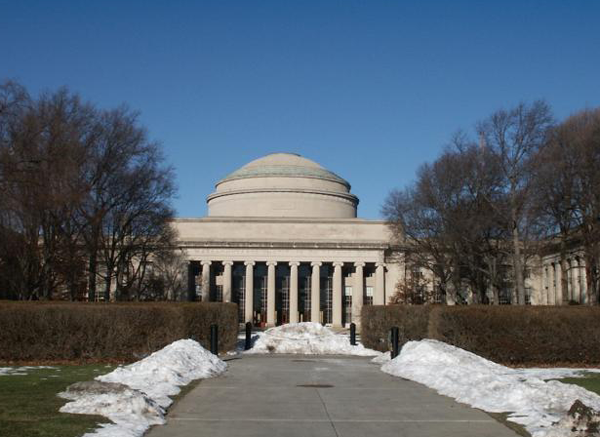
\includegraphics[width=0.9\columnwidth]{Figure1}
% \caption{With Caption Below, be sure to have a good resolution image
%   (see item D within the preparation instructions).}
% \label{fig:figure1}
% \end{figure}

% \begin{table}
%   \centering
%   \begin{tabular}{|c|c|c|}
%     \hline
%     \tabhead{Objects} &
%     \multicolumn{1}{|p{0.3\columnwidth}|}{\centering\tabhead{Caption --- pre-2002}} &
%     \multicolumn{1}{|p{0.4\columnwidth}|}{\centering\tabhead{Caption --- 2003 and afterwards}} \\
%     \hline
%     Tables & Above & Below \\
%     \hline
%     Figures & Below & Below \\
%     \hline
%   \end{tabular}
%   \caption{Table captions should be placed below the table.}
%   \label{tab:table1}
% \end{table}



% Balancing columns in a ref list is a bit of a pain because you
% either use a hack like flushend or balance, or manually insert
% a column break.  http://www.tex.ac.uk/cgi-bin/texfaq2html?label=balance
% multicols doesn't work because we're already in two-column mode,
% and flushend isn't awesome, so I choose balance.  See this
% for more info: http://cs.brown.edu/system/software/latex/doc/balance.pdf
%
% Note that in a perfect world balance wants to be in the first
% column of the last page.
%
% If balance doesn't work for you, you can remove that and
% hard-code a column break into the bbl file right before you
% submit:
%
% http://stackoverflow.com/questions/2149854/how-to-manually-equalize-columns-
% in-an-ieee-paper-if-using-bibtex
%
% Or, just remove \balance and give up on balancing the last page.
%
\newpage
\balance

% REFERENCES FORMAT
% References must be the same font size as other body text.

\bibliographystyle{acm-sigchi}
\bibliography{masterthesis-pape}


\clearpage
\newpage
\onecolumn

\begin{landscape}


\section{Appendix A. Semi-Structured Interview and Expert Interview Guidelines}
\subsubsection{Appendix A.1. Semi-Structured Interview Guideline (in German)}
The interview guideline was developed following rules of Helfferich \cite{helfferich2005}. It is in german as the interviews were held in german. Participants were shown the developed application prior to the interview.
\begin{adjustwidth}{-8em}{-8em}

\begin{longtable}{|p{6.45cm}|p{6.45cm}|p{6.45cm}|p{6.45cm}|}
 \hline
 \textbf{Leitfrage (Erz{\"a}hlaufforderung)}&\textbf{Check -- Wurde das erw{\"a}hnt? Memo f{\"u}r m{\"o}gliche Nachfragen -- nur stellen wenn nicht von allein angesprochen! Formulierung anpassen}&\textbf{Konkrete Fragen -- bitte an passender Stelle (auch am Ende m{\"o}glich) in dieser Formulierung stellen}&\textbf{Aufrechterhaltungs- und Steuerungsfragen}\\
 \hline

 \multicolumn{4}{|l|}{\textbf{Teil 1 -- B{\"u}rgerbeteiligung}}\\
 \hline
 
 Erz{\"a}hlen Sie mir {\"u}ber ihre Rolle und Aufgaben in B{\"u}rgerbeteiligung & Wie lange aktiv (Befragter, Projekt)\newline "`Organisator"' oder "`an der Basis"' & & Erz{\"a}hlen Sie noch mehr {\"u}ber\dots \\
 \hline
 
 
 Bitte beschreiben Sie mir die aus ihrer Sicht wichtigsten Aspekte von B{\"u}rgerbeteiligung. & Ziele \newline Nutzen & & \\
 \hline
 
 Bitte geben Sie mir eine Einf{\"u}hrung in ein(e) laufende(s)/ abgeschlossene(s) Initiative/Projekt (spontan entscheiden welches mehr "`dialogische"' Interaktion zwischen B{\"u}rgern und Aktion erfordert)& Methoden f{\"u}r B{\"u}rgerbefragung \newline Wie erfolgreich/Probleme? \newline "`Moderne"' (Social media) methoden angedacht? \newline Form von Beitr{\"a}gen die B{\"u}rger gebracht haben \newline Wie wurden die Aspekte ber{\"u}cksichtigt?
   & Welchen Wert wurde auf Dialoge zwischen den Akteuren gelegt? & Wie ist das ganze dann abgelaufen?\\
 \hline
 
 \multicolumn{4}{|l|}{\textbf{Teil 2 -- Einsatz der Anwendung}}\\
 \hline
 
 Bitte geben Sie mir eine Einf{\"u}hrung in das Projekt in dem Sie die Anwendung einsetzen wollen. & Zielgruppe (Bev{\"o}lkerungsgruppen, Geographisch) \newline redaktionelle Inhalte \newline erwartete Inhalte \newline Anreize zu Dialogen/Austausch mit B{\"u}rgern? & K{\"o}nnen Sie sich weitere Anwendungsf{\"a}lle f{\"u}r die Verkn{\"u}pfung von Texten mit Karten neben B{\"u}rgerbeteiligung vorstellen? & Erz{\"a}hlen Sie noch mehr {\"u}ber\dots \\
 \hline
 
 Welche Gr{\"u}nde sprechen f{\"u}r den Einsatz dieser L{\"o}sung gegen{\"u}ber anderen L{\"o}sungen. & Bedingungen (technisch, funktional) \newline angedachte Alternativen und deren Defizite \newline B{\"u}rgerbeteiligungsaspekte ber{\"u}cksichtigt? & Welche Eigenschaften w{\"u}rden Sie davon abhalten solch eine Anwendung einzusetzen? \newline Was k{\"o}nnte B{\"u}rger davon abhalten sich durch die Anwendung zu beteiligen? & \\
 \hline

 \multicolumn{4}{|l|}{\textbf{Teil 3 -- Abschlie{\ss}ende Fragen}}\\
 \hline
 
 Kennen Sie Beispiele f{\"u}r die Verkn{\"u}pfung geographischer Daten mit Diskussionsbeitr{\"a}gen? & Next Kassel/Hamburg \newline Frankfurt Gestalten \newline Shareabouts \newline collaborativemap.org & & \\
 \hline
 
 Haben Sie sich dort beteiligt? & In welcher Form & & Wie ist das ganze dann abgelaufen? \\
 \hline
 
 Kennen Sie Werkzeuge um interaktive Karten mit eigenen Inhalten zu erzeugen? & Google Map Maker \newline Here Map Creator \newline Wikimapia \newline Unclemap & & \\
 \hline
 
 Haben Sie schonmal ein solches Werkzeug eingesetzt? & Wie? & &\\
 \hline
 
 \end{longtable}
\end{adjustwidth}
\end{landscape}
\newpage

\subsubsection{Appendix A.1. Expert Interview Guideline}

As mentioned by Helfferich \cite{helfferich2005}, can handle more direct questions. Therefore these questions are much more straightforward. Because the interviews were held in german, the questions are also in german. Prior to the interview, the developed application was demoed.
\begin{itemize}
    \item Kennen Sie Anwendungen die Diskussionen durch Geoobjekte unterst{\"u}tzen?
    \item Welche davon haben Sie in der Vergangenheit schon einmal benutzt?
    \item Z{\"a}hlen Sie bitte die Vor- und Nachteile dieser Anwendungen auf
    \item Welche Anwendungsf{\"a}lle f{\"u}r die Verkn{\"u}pfung von Diskussionen und Geoobjekten k{\"o}nnen Sie sich außerhalb des B{\"u}rgerbeteiligungskontextes vorstellen?
    \item Welche L{\"o}sungen um B{\"u}rger mit Initiativen/Politik zusammenzubringen kennen Sie?
    \item Wie l{\"a}uft die Kommunikation zwischen den B{\"u}rgern und Initiativen/Politik bei diesen L{\"o}sungen ab?
    \item Denken Sie die explizite Verkn{\"u}pfung von Geoobjekten mit Diskussionsgegenst{\"a}nden ist generell hilfreich im B{\"u}rgerbeteiligungskontext / bei Dialogen?
    \item Im Vergleich zu den Anwendungen die Sie kennen, was denken Sie {\"u}ber die folgenden Funktionen der eben vorgestellten Anwendung?
        \begin{itemize}
            \item Verstecken von Geoobjekten die zu Antworten erstellt worden sind; In der Themenansicht nur die Geoobjekte der initialen Beitr{\"a}ge auf der Karte
            \item Zwei Wege Highlights von Geoobjekten und Beitr{\"a}gsboxen
            \item Filter und Sortierung
            \item Verfassen/Antworten
            \item Verkn{\"u}pfen von W{\"o}rtern mit neuen Geoobjekten, bestehenden Geoobjekten und Links
            \item Favorisierung von Beitr{\"a}gen
            \item Benutzerregistrierung/Anmeldung (und Social Login)
        \end{itemize}
    \item Werden ihrer Meinung nach Dialoge vereinfacht oder unterst{\"u}tzt?
    \item Welche Funktionen haben Sie vermisst?
    \item Was k{\"o}nnte B{\"u}rger davon abhalten sich durch die Anwendung zu beteiligen?

\end{itemize}

\twocolumn
\section{Appendix B. Transcribed Interviews}

\subsubsection{Appendix B.1. Transcription System}
The interviews and the focus group were transcribed the following these rules (Rules from Kuckarz \cite{kuckartz2007} with modifications):
\begin{enumerate}
    \item The transcription is literal. Dialects are not transcribed.
    \item Punctuation and language are modified to match grammar and syntax of the german language.
    \item All personal details and mentions are removed and anonymized to prevent re-identification.
    \item Pauses and breaks are marked with ellipses (\dots).
    \item Agreeing sounds like ``Mhms'', ``Ahas'', etc. of the interviewer are not transcribed if they did not interrupt the interviewee.
    \item Interjections of the other person are in brackets.
    \item Supporting or clarifying sounds of the interviewee like laughing or sighing are noted in brackets.
    \item Passages of the interviewing person are denoted with ``I:'', passages of the interviewed person with a distinct abbreviation like ``P1:''.
\end{enumerate}

\subsubsection{Appendix B.2. Demo and Introduction to the Application}

In each interview, the interviewer introduced and demoed the application to the interviewed person. This exemplary introduction was transcribed from the interview with participant 1. In order to retain bevity, it is omited in the other transcriptions.

In each interview, the interviewer introduced and demoed the application to the interviewed person. This exemplary introduction was transcribed from the interview with participant 1. In order to retain brevity, it is omitted in the other transcriptions.

\begin{itemize}
\item[I:] Hallo, erstmal vielen Dank, dass Sie sich hier Zeit f{\"u}r mich und meine Masterarbeit nehmen. Es soll jetzt gleich hier um die von mir entwickelte Anwendung gehen. Danach werde ich ihnen noch ein paar Fragen stellen. Also meine Masterarbeit hat das Thema "`Supporting public deliberation through spatially enhanced dialogs"'. Das bedeutet grob, dass ich herausfinden will wie man Dialoge in der B{\"u}rgerbeteiligung durch kartenbasierte Anwendungen unterst{\"u}tzen kann. Also, ich fange dann einfach mal mit der Demo der Anwendung an. (ruft die Anwendung auf) Wenn man als Benutzer auf die Webseite kommt, dann wird man beim ersten Besuch erstmal hier mit so einem Text begr{\"u}{\ss}t, der erstmal ein bisschen das Thema vom Nachhaltigkeitstag erkl{\"a}rt. Bei der Entwicklung der Karte wurde ich von Mitgliedern des "`Arbeitskreis Gemeinsam Nachhaltig"' unterst{\"u}tzt. Die sind vom Institut f{\"u}r Soziologie hier in M{\"u}nster. Das sah dann so aus, dass wir uns an mehreren Treffen {\"u}ber die Entwicklung der Anwendung unterhalten haben. Die Soziologen haben mir dann ihre Meinung und Ideen gesagt, die ich dann versucht habe umzusetzen. Also letztendlich soll wohl wahrscheinlich die Anwendung dann n{\"a}chstes Jahr in dem geplanten Nachhaltigkeitstag eingesetzt werden. (klickt auf weiter) Hier kriegt man so kleine Einf{\"u}hrungsvideos, aber das mache ich ja jetzt m{\"u}ndlich, da brauchen wir uns die nicht anschauen. (klickt weiter) Dann hier die Zeichenerkl{\"a}rung f{\"u}r die Marker in der Karte. Man sieht ja hier, dass es zwei Dimensionen gibt. Das sind hier die Akteure, gekennzeichnet durch die Farbe und dann die Aktivit{\"a}t durch den Buchstaben im Marker. (f{\"a}hrt mit der Maus {\"u}ber die Tabellenzellen) Hier kann man sich dann noch kleine Erkl{\"a}rungen zu den Akteuren und Aktivit{\"a}ten durchlesen. (klickt auf weiter) Dann gibts hier noch einen Text zum Kontext der Anwendung. (klickt auf "`Alles klar, ich will loslegen!"') So dann sind wir hier jetzt in der {\"U}bersicht der Anwendung. Man sieht direkt die Karte und am rechten Rand gibts noch so eine Seitenleiste. In der Seitenleiste finden sich die Beitr{\"a}ge, ein Filter und die Eingabemaske f{\"u}r das Einstellen von neuen Themen. (f{\"a}hrt mit der Maus {\"u}ber einen Marker) Hier wenn man jetzt mit der Maus {\"u}ber so einen Marker f{\"a}hrt, dann sieht man direkt, dass der Marker visuell hervorgehoben wird. Also der orangene Ring und das Popup. Gleichzeitig wird der zugeh{\"o}rige Beitrag in der Seitenleiste hervorgehoben, damit man direkt sehen kann, zu welchem Beitrag der Marker geh{\"o}rt. (f{\"a}hrt mit der Maus {\"u}ber einen Beitrag in der Seitenleiste) Das ganze funktioniert dann auch in der anderen Richtung. Man kann direkt dann sehen welche Marker zu dem Beitrag geh{\"o}ren. (klickt auf einen Beitrag in der Seitenleiste) So dann kann man die Beitr{\"a}ge hier noch so ausklappen, um dann auch den Beschreibungstext lesen zu k{\"o}nnen. Ja also neben dem Beschreibungstext kann man dann hier auch lesen von wann der Beitrag ist und wer ihn geschrieben hat. Sonst sind hier noch der Akteur, Aktivit{\"a}t und Inhalte zu lesen. Dann gibts hier noch dieses Herzchen mit der Zahl davor. Das zeigt an wie oft der Beitrag von den Benutzern favorisiert worden ist. Das ist so {\"a}hnlich wie ein Facebook "`Gef{\"a}llt mir"'. (tippt ein paar Buchstaben in den Filter) So dann gibts hier noch den Filter. Hier kann man entweder direkt nach einem Wort suchen, oder dann mit den Filteroptionen (klickt auf "`Filter einblenden"') entweder nach Akteur, Aktivit{\"a}t oder Inhalt filtern. Hier ganz unten gibts noch die Filteroption "`Zeitraum unbegrenzt"'. Das ist noch ne Besonderheit. Die Beitr{\"a}ge k{\"o}nnen ein Ablaufdatum bekommen. Dann werden die nach Ablauf des Ablaufdatums dann auch nicht mehr auf der Karte und in der Seitenleiste angezeigt. Hier mit der Option kann man sie dann wieder einblenden. (klickt auf "`alle Filter zur{\"u}cksetzen"' und dann auf "`Filter ausblenden"') So und dann kann man noch hier noch die Sortierreihenfolge in der Seitenleiste ver{\"a}ndern. Da kann man dann sortieren wie man die Beitr{\"a}ge hier gerne h{\"a}tte. Achso, hier in den Beitr{\"a}gen kann man dann auch schon sehen wie viele Antworten das Thema schon hat. (klickt auf "`Antworten anzeigen"') Wie Ihnen wahrscheinlich schon aufgefallen ist, hat sich nicht nur der Kartenausschnitt ver{\"a}ndert, sondern es werden jetzt auch andere Marker als gerade angezeigt. Das ist auch so ne Besonderheit. In der {\"U}bersicht werden nur die Marker angezeigt, die zu den initialen Beitr{\"a}gen der Themen erstellt worden sind. Das ist damit die Karte nicht zu schnell zu voll wird, und man noch den {\"U}berblick hat. Hier in den Antworten k{\"o}nnen Sie ja sehen, da sind so unterschiedlich farbige Boxen. Die gr{\"u}nen zeigen an, dass da ein Marker verlinkt worden ist, die braunen zeigen, dass ein bestehender Marker referenziert worden ist, und blau bedeutet, dass dort eine Webseite verlinkt worden ist. Also schreiben wir jetzt einfach mal eine Antwort. (klickt auf "`Antwort verfassen"') Hier hat sich jetzt die Eingabemaske f{\"u}r Antworten ausgeklappt. Da kann man nur eine Beschreibung mit Geoobjekten, referenzierten Geoobjekten und Link angeben und ein Bild anh{\"a}ngen. Der Rest Attribute wie Akteur und so werden vom Thema geerbt. (tippt eine Beschreibung) So nachdem man nun seinen Text verfasst hat, kann man noch W{\"o}rter verlinken. Das geht wie gesagt mit einem neuen Marker, einem bestehenden Marker, oder einem Link zu einer Webseite. Dazu muss man hier ein Wort oder halt mehrere W{\"o}rter markieren. (markiert ein Wort mit der Maus) Dann sieht man hier so ein Kontextmen{\"u} mit drei Buttons. Der erste ist f{\"u}r einen neuen Marker, der zweite um einen bestehenden Marker zu verkn{\"u}pfen und der dritte um eine Webseite zu verlinken. (klickt auf den "`Marker"'-Button) Ich mach jetzt hier mal einen neuen Marker. (klickt in die Karte) So jetzt wurde das Wort und der Ort, an dem ich den Marker gesetzt habe, verkn{\"u}pft. (markiert ein anderes Wort und klickt auf den "`Verkn{\"u}pfen"'-Button) Genauso funktioniert das dann auch mit dem Verkn{\"u}pfen. (klickt auf einen bestehenden Marker in der Karte). Und dann nochmal mit der Webseite (markiert ein drittes Wort und klickt auf den "`Link"'-Button) Hier beim Webseiten verlinken {\"o}ffnet sich dann so ein kleines Eingabefeld wo man dann den Link reinschreiben kann. (schreibt einen Link in das Feld und dr{\"u}ckt die Enter-Taste auf der Tastatur) So lange man die Antwort noch nicht abgeschickt hat, kann man auch noch alles l{\"o}schen und dann ist es auch weg. Sp{\"a}ter beim Editieren geht das nicht mehr. So wenn man jetzt noch ein Bild hat, kann man das hier unten anh{\"a}ngen noch. Das funktioniert aber so wie man es erwartet, ich hab jetzt auch keines gerade. (klickt auf "`Abschicken"') So, da man noch nicht eingeloggt, ist kann man nat{\"u}rlich den Beitrag jetzt noch nicht abschicken. Also verfassen geht, abschicken aber nicht. Da kommt man dann hier zu dem Login-Dialog. Hier kann man sich entweder mit Facebook, Twitter oder Google einloggen, oder halt auch ganz traditionell mit E-Mail und Passwort wenn man sich vorher hier auch registriert hat. (loggt sich ein). Dann kann man jetzt auch die Antwort abschicken. So wenn man jetzt merkt, dass man sich verschrieben hat oder dass der Marker falsch ist, kann man jetzt den Fehler korrigieren. Dazu muss man hier auf den kleinen Stift dr{\"u}cken, (klickt auf den Stift) und kann dann den Beitrag bearbeiten. ({\"a}ndert einen Buchstaben, verschiebt den Marker und {\"a}ndert den Link) Man kann das hier durch draufklicken auf den kleinen Kasten ausl{\"o}sen, das {\"a}ndern des Links. (klickt auf "`Abschicken"') So jetzt sind die {\"A}nderungen gespeichert, und man kann direkt sehen, dass jetzt hier auch "`ge{\"a}ndert am"' steht. So dann gibts hier noch den Button mit der kleinen Tonne. Damit kann man den Beitrag l{\"o}schen. Editieren und l{\"o}schen geht nat{\"u}rlich nur bei Beitr{\"a}gen, von denen man selber der Autor ist. Das l{\"o}schen ist dann auch kein richtiges L{\"o}schen, sondern da kann man dann einen Grund angeben, warum der Beitrag gel{\"o}scht werden soll. (klickt auf die kleine Tonne) Also hier kann man den Grund angeben (tippt Grund ein und klickt auf "`Ja, Beitrag l{\"o}schen"') So dann sieht man direkt dass der Beitrag ausgegraut wird, durchgestrichen und dann auch noch die Marker in hellerer Farbe dargestellt werden. Man kann nicht komplett l{\"o}schen, weil sonst der Sinn von den Diskussionen verloren gehen k{\"o}nnte. Die Themenstarter kann dann auch nichtmal der Autor l{\"o}schen. So wenn man denn nun jetzt nicht der Autor eines Beitrages ist, dann kann man hier mit dem kleinen Herzchen den Beitrag favorisieren. (klickt auf das Herzchen) Dann sieht man auch direkt, die Zahl hier unten neben dem anderen Herzchen erh{\"o}ht sich und das Herzchen wird ausgef{\"u}llt. Das bedeutet, dass man selbst den Beitrag favorisiert hat. Das ganze kann man dann nat{\"u}rlich auch wieder entfavorisieren wenn man wieder auf das kleine Herzchen klickt. (klickt auf den "`zur{\"u}ck"'-Button) So okay, dann wollen wir auch nochmal ein neues Thema erstellen. (klickt in das "`Titel"'-Feld) So hier hat sich jetzt die Eingabemaske f{\"u}r neue Themen ausgeklappt. Hier kann man dann den Titel, einen Akteur, eine Aktivit{\"a}t und mehrere Inhalte ausw{\"a}hlen. Dann kann man hier einen Start- und Endzeitpunkt ausw{\"a}hlen.  Darunter, das kennen Sie ja schon von eben, kann man eine Beschreibung eingeben und darunter noch ein Bild anh{\"a}ngen. (f{\"u}llt die Felder aus und klickt "`Abschicken"') So und dann hat man hier ein neues Thema. Hier unten auf der Seite kommt man dann auch nochmal zu der Zeichenerkl{\"a}rung, und hier oben nochmal zu den Erkl{\"a}rungsvideos. Ja also das war es jetzt erstmal zur Anwendung.
\end{itemize}

\subsubsection{Appendix B.3. Participant 1}

\textbf{Teil 1 -- B{\"u}rgerbeteiligung}
\begin{itemize}
    \item[I:] Erz{\"a}hlen Sie mir {\"u}ber ihre Rolle und Aufgaben in B{\"u}rgerbeteiligung
    \item[P1:] Ich kann nur sagen was f{\"u}r mich wichtig ist
    \item[I:] Ja das ist auch eine Sache die Sie mir erz{\"a}hlen k{\"o}nnen. Dann beschreiben Sie mir bitte die aus ihrer Sicht wichtigsten Aspekte der B{\"u}rgerbeteiligung
    \item[P1:] Die B{\"u}rgerbeteiligung f{\"u}hrt dazu, das erstmal Leute sich informieren, dass sie mehr wissen als nur {\"u}ber Zeitung. Dann k{\"o}nnen sie sich auch zusammenschlie{\ss}en und diskutieren und Aktionen besprechen. Ja und auch entsprechend Aktionen machen. Das st{\"a}rkt auch im Grunde eine Stadt.
    \item[I:] An welchen B{\"u}rgerbeteiligungsaktionen haben Sie dann schonmal teilgenommen?
	\item[P1:] Ja die Frage ist jetzt was alles unter B{\"u}rgerbeteiligung f{\"a}llt?
	\item[I:] Da kann alles drunter fallen, was f{\"u}r die {\"O}ffentlichkeit geschieht.
	\item[P1:] Also, ich habe zum Beispiel mit Leuten zusammen einen Gemeinschaftsgarten, der ist gegr{\"u}ndet worden und da treffen wir uns, da wird Gem{\"u}se angebaut, da gibts Bienen und da ist auch gedacht, dass man sich noch in Zukunft wenn das mal l{\"a}uft sich vernetzt mit anderen G{\"a}rten. Zum Beispiel zum Thema Bienen haben wir einen Nachmittag gehabt. Aber das kann man nat{\"u}rlich auch in einen gr{\"o}{\ss}eren Ma{\ss}stab machen.
	\item[I:] Und w{\"u}rden Sie denken, dass in diesem Kontext so eine Art von geographischer Diskussions-Anwendung dann sinnvoll einzusetzen w{\"a}re um das ganze bekannter zu machen und die Inhalte nach au{\ss}en zu kommunizieren?
	\item[P1:] Ja erstmal stell ich mir das so vor, dass jemand der, meinetwegen, neu ist oder keine Kontakte hat, sich mit Hilfe der Karte {\"u}berhaupt mal ein Bild machen was es f{\"u}r M{\"o}glichkeiten gibt. Und dann geht es ja in die Feindifferenzierung. Da w{\"u}rde er sagen: "`Gut, ich interessiere mich f{\"u}r Umwelt. Wer ist zust{\"a}ndig f{\"u}r Umwelt. Naja Greenpeace kann ich mal anklicken. Wo treffen die sich. Wann treffen die sich. Was haben die f{\"u}r Aktivit{\"a}ten zum Beispiel. Oder Transition Town. Was machen die eigentlich. Muss ich mal lesen was das {\"u}berhaupt ist. Ich wei{\ss} gar nicht genau was das ist. Also kann ich das mal lesen und vielleicht auch Kontakt aufnehmen."' Ich muss mir jetzt nicht m{\"u}hsam diese ganzen Adressen zusammensuchen. Diese WWW-Adressen, sondern die sind ja auf deiner Karte schon angegeben. Das ist nat{\"u}rlich schon auch erleichternd ist. Denn manchmal scheitert es an solchen Sachen. Auch an Bequemlichkeit.
	\item[I:] Wie l{\"a}uft dann im Moment die Kommunikation intern f{\"u}r diesen Garten ab?
	\item[P1:] {\"U}ber E-Mail und {\"u}ber Treffen.
	\item[I:] Wie oft treffen sie sich da?
	\item[P1:] Ja da gibts dann Einladungen. Aber das ist unterschiedlich. Alle zwei Monate wenn was ansteht. Jetzt wo das Wasser da ist, da trifft man sich mal um aufzur{\"a}umen oder um Projekte zu besprechen.	
\end{itemize}

\textbf{Teil 2 -- Einsatz der Anwendung}
\begin{itemize}
	\item[I:] Wie soll dann die Beteiligung von Transition Town oder dem Garten auf dem Nachhaltigkeitstag aussehen?
	\item[P1:] Naja das kann ich jetzt nur erfinden. Letztenendes m{\"u}ssen wir das ja als Gruppe besprechen.
	\item[I:] Also am besten wie Sie sich das vorstellen
	\item[P1:] Themen die Transition Town wichtig sind w{\"u}rden da einen Raum finden und den Rahmen m{\"u}ssen die sich dann geben. Ob das jetzt in Form von (\dots) dass man gesundes Essen anbietet, oder mal so ne Karte entwirft wo Transition Town ist. Es gibt ja auch einen Film {\"u}ber Transition Town. Da gibts ja vielf{\"a}ltige M{\"o}glichkeiten. (\dots) Zum Beispiel in unserem Garten da hat die Bienen-Frau einen Vortrag gehalten {\"u}ber die Bienen und das soziale Miteinander. Das ist ja hoch differenziert. Zum Beispiel die Drohnen, die treffen sich an ganz bestimmten Pl{\"a}tzen vierzig Meter {\"u}ber der Erde. Solche die Detailinformationen die kein Mensch eigentlich wei{\ss}, die k{\"o}nnte man dann geben, in dem diese Bienen-Frau vielleicht was mitbringt und dann dar{\"u}ber redet und das dann auch Kindern zeigt wie so ein Bienenstock aussieht und mal Honig probieren l{\"a}sst. Und dann auch zum engagieren auffordert. Oder hab ich heute in der Zeitung gelesen, dass es einen Jungen gibt, der hat ein Bienenhaus gebaut f{\"u}r den Balkon. Der w{\"u}rde dann eingeladen und w{\"u}rde das vorstellen.
	\item[I:] Wer w{\"a}re dann die Zielgruppe? 
	\item[P1:] Wie meinst du die Zielgruppe?
	\item[I:] Ich meine damit die Personenkreise die man ansprechen m{\"o}chte
	\item[P1:] Naja an dem Tag werden ja viele Menschen da sein. Und das w{\"a}re ja dann ein wichtiger Aspekt zum Nachhaltigkeitsthema. Ich meine, da dass ja wahrscheinlich drau{\ss}en stattfindet, kann man ja von Zielgruppe nicht so unbedingt sprechen, oder? Wer will, der kommt.
	\item[I:] Gibt es andere Ans{\"a}tze die Sie zur Kommunikation bez{\"u}glich des Nachhaltigkeitstages in Betracht gezogen haben?
	\item[P1:] Nein im Moment nicht.
	\item[I:] Was f{\"u}r Gr{\"u}nde w{\"u}rden f{\"u}r den Einsatz der Karte sprechen? 
    \item[P1:] Also du meinst was f{\"u}r Vorteile es f{\"u}r uns h{\"a}tte den Garten in deine Karte einzutragen?
    \item[I:] Richtig.
	\item[P1:] Das h{\"a}tte den Vorteil, dass man auf einen Blick sehen kann, da und da und da gibt es einen freien Garten. Man sieht welche Adresse das sind. Man sieht vielleicht auch wann die da sind. Und dann ist das nat{\"u}rlich sehr {\"u}bersichtlich. Mit einem Klick hat man sozusagen die Information. Es gibt ja noch mehrere G{\"a}rten. Es gibt da unseren Paradies-Garten, dann gibt es am Campus noch einen Garten, dann gibts noch an der Gasselstiege einen Garten. Ja. Die w{\"u}rde man dann da sehen und dann k{\"o}nnte man auch Leute die das wollen, meinetwegen, eine Fahhradtour machen lassen und die G{\"a}rten angucken. Man k{\"o}nnte die  Karte auch benutzen um die Fahrradtour zu organisieren. Dass man Start, Ziel und Zwischenhalte markiert.
	\item[I:] Was k{\"o}nnten Sachen sein die B{\"u}rger davon abhalten w{\"u}rden diese Karte zu benutzen?
	\item[P1:] (\dots) Ja also die Karte ist ja elektronisch. Geht ja nur {\"u}ber das Internet. Also sofern man einen Internetanschluss hat und einen Laptop oder einen Computer, gibts da nichts was dagegen spricht.
\end{itemize}
\textbf{Teil 3 -- Abschlie{\ss}ende Fragen}
\begin{itemize}
    \item[I:] Kennen Sie Beispiele f{\"u}r die Verkn{\"u}pfung geographischer Daten mit Diskussionsbeitr{\"a}gen?
	\item[P1:] Sag mir nochmal was man alles unter geographische Daten fasst.
	\item[I:] Orte und Objekte mit einem Ort
	\item[P1:] Naja ich war jetzt auf dem Jakobsweg, da hat man auch Karten. Aber die nutzt man nicht so oft. Da hat man B{\"u}cher in denen die Adressen drin stehen. Und die Zeichen sind an den B{\"a}umen.
	\item[I:] Ja ist auch ne M{\"o}glichkeit. Ich ziele mit der Frage eher ab auf auf elektronische Anwendungen.
	\item[P1:] Nein, ich nicht da auch nicht so firm. Ich mag das auch nicht.
	\item[I:] Also haben Sie sowas auch noch nie benutzt?
	\item[P1:] Nein.
	\item[I:] Kennen Sie Werkzeuge um interaktive Karten mit eigenen Inhalten zu erzeugen?
	\item[P1:] Nein. Es gibt ja viele Leute die nicht so interessiert sind mit den neuen Medien. 
	\item[I:] Ja. Alles klar. Das waren dann die Fragen von meiner Seite. Gibt es noch Fragen von ihrer Seite? 
    \item[P1:] Nein. Eigentlich nicht. Gute Sache.
    \item[I:] Vielen Dank f{\"u}r ihre Zeit.
\end{itemize}

\subsubsection{Appendix B.4. Participant 2}

\textbf{Teil 1 -- B{\"u}rgerbeteiligung}
\begin{itemize}
    \item[I:] Erz{\"a}hlen Sie mir {\"u}ber ihre Aufgaben und Rollen in der B{\"u}rgerbeteiligung
    \item[P2:] Also das ist eine schwierige Frage, weil ich da gar nicht so Aufgaben oder Rollen habe sondern mir sie eher selbst suche. Das hei{\ss}t, ich mache meistens das, was ich interessant finde. Und jetzt in dem Kontext halt zum Beispiel, diese Organisation des Nachhaltigkeitstages und in dem Kontext dann auch die Arbeit mit der Karte.
    \item[I:] Und wie lange sind Sie da jetzt schon aktiv? 
    \item[P2:] Es hat, denke ich, so angefangen mit der Organisation der Tagung. Vor allem in letzter Zeit wieder mehr. (War das letztes Jahr?) Ja, letztes Jahr. Oder es hat 2012 angefangen. Wahrscheinlich sogar eher Ende 2011 oder so. Aber davor war ich aber auch schonmal so in dem Bereich, w{\"a}hrend des Studiums unterwegs. So NGOs und Entwicklungszusammenarbeit und sowas.
    \item[I:] Bitte beschreiben Sie mir aus ihrer Sicht wichtige Aspekte der B{\"u}rgerbeteiliung.
    \item[P2:] Beteiligung. (lacht) Also, das ist nat{\"u}rlich erstmal ein theoretisches Konzept, aber in der Praxis w{\"u}rde ich sagen, ist das wichtige, dass die Leute wirklich mitmachen und mitgestalten. Das hei{\ss}t, nicht nur passiv so da sitzen, sondern halt eine aktive Rolle haben.
    \item[I:] Und die Ziele und Nutzen davon?
    \item[P2:] Ja, die Ziele und Nutzen sind erstmal so eine Art von Legitimation von Ma{\ss}nahmen, w{\"u}rde ich sagen. Dabei w{\"u}rde ich nichtmal sagen dass das der Hauptpunkt ist, sondern eigentlich dass den Menschen die M{\"o}glichkeit gegeben wird, ihr eigenes Umfeld so zu gestalten, wie sie es gerne wollen. Und, dass sie in dem Umfeld, wo sie leben nicht so beschr{\"a}nkt sind von {\"a}u{\ss}eren Sachen. Sondern halt eher selbstbestimmt alles zu organisieren.
    \item[I:] Bitte geben Sie mir eine Einf{\"u}hrung in das Nachhaltigkeitsprojekt.
    \item[P2:] Also im Prinzip hat es, wie gesagt, schon begonnen mit der Tagung letztes Jahr. Das war der Startschuss, dass wir uns gedacht haben, nach dieser Tagung muss es eigentlich irgendwie weitergehen. Das haben damals auch alle gesagt, dass man danach einen Nachfolgeprozess organisieren wollte. Dazu haben wir dann ein paar Treffen nach der Tagung gemacht. Auf diesen Treffen haben wir dann entschieden, dass wir so einen Tag der Nachhaltigkeit organisieren, was dahin f{\"u}hren soll, dass n{\"a}chstes Jahr, am 15. Juni 2015 ein Tag in M{\"u}nster stattfindet, an dem an verschiedenen Orten Nachhaltigkeitsprojekte vorgestellt werden und {\"o}ffentlich {\"u}ber das Thema diskutiert werden kann. Dazu soll dann auch vorher ein bisschen {\"O}ffentlichkeitsarbeit in den Medien gemacht werden. Das hei{\ss}t, dass man versucht, den Diskurs somit weiter zu befeuern um das Projekt im Bewusstsein zu halten. Das ist auch dann das Hauptanliegen im Moment.
    \item[I:] Wieviel Wert wurde da im Vorfeld auf Dialoge gelegt?
    \item[P2:] Es kommt drauf an. Wir haben auf dieser Tagung eine Mailingliste angelegt, so dass wir jetzt verschiedene Verteiler haben. Das ist jetzt dann aber nicht f{\"u}r die gesamte {\"O}ffentlichkeit, sondern eher f{\"u}r diesen Kreis, der auch da auf der Tagung war. Gleichzeitig haben wir auch {\"u}ber Zeitungsartikel und Einladungen in den Medien versucht, Leute zu mobilisieren au{\ss}erhalb des Kreises. Das war allerdings nicht sehr erfolgreich. Insofern versuchen wir das demn{\"a}chst auch nochmal im Oktober oder so, aber haben jetzt noch nicht gezielt auf Breitenbeteiligung geschaut.
    \item[I:] Habt ihr euch im Vorfeld schon nur auf Zeitung festgelegt oder gab es auch in Richtung Social Media vorschl{\"a}ge?
    \item[P2:] Nein, das wurde eher spontan entschieden. Da war nur die Entscheidung, dass wir unsere eigenen Netzwerke aktivieren. Das war der eine Pfad und der andere w{\"a}re halt, {\"u}ber Medien die breitere {\"O}ffentlichkeit zu erreichen. Also {\"u}ber Social Media haben wir, glaube ich, gar nicht geworben. Nur halt E-Mail-m{\"a}{\ss}ig {\"u}ber die Listen.
\end{itemize}

\textbf{Teil 2 -- Einsatz der Anwendung}
\begin{itemize}
    \item[I:] Dann geht es jetzt weiter konkret zur Anwendung. Wer ist die Zielgruppe f{\"u}r die Anwendung?
    \item[P2:] Also die Zielgruppe sind potentiell eigentlich erstmal alle Interessierten. Ich w{\"u}rde das gar nicht so eingrenzen wollen. Nat{\"u}rlich in der Praxis sind das dann meistens diejenigen, die sowieso engagiert sind und in dem Bereich arbeiten.
    \item[I:] Was f{\"u}r Inhalte erwarten Sie?
    \item[P2:] Ich geh mal erstmal vom Idealfall aus. Ideal w{\"a}re es, wenn sich die Leute, die sowieso schon aktiv in ihren Bereichen sind, der Karte annehmen w{\"u}rden und dar{\"u}ber die Strukturen der Beteiligung in M{\"u}nster im Bereich Nachhaltigkeit einfach digital sichtbar machen w{\"u}rden, von allein. Das w{\"a}re dann so eine Form der Datenerhebung in einer gewissen Art und Weise. Das w{\"a}re dann so der Idealfall, wenn dann {\"u}ber diese Prozesse dann Kommunikation in Gang kommt. Das sollte dann auch m{\"o}glichst weit streuen, {\"u}ber m{\"o}glichst viele Schichten und Stadtbezirke und so weiter. Das hei{\ss}t, dass sich dann so ein Synergieeffekt ergibt. Realistisch gesehen wird es wahrscheinlich nicht ganz so weit gehen, denke ich. Deswegen w{\"a}re vielleicht so der erste Punkt, dass das anl{\"a}uft, dass sich andere beteiligen. Das w{\"a}re schon ein erster kleiner Schritt, dass es {\"u}ber den Kreis, die da sowieso schon mitmachen, hinaus bekannter wird.
    \item[I:] K{\"o}nnen Sie sich weitere Anwendungen f{\"u}r die Verkn{\"u}pfung von Geoobjekten mit Karten neben der B{\"u}rgerbeteiligung vorstellen?
    \item[P2:] Sicherlich. Da k{\"o}nnte man einfach erstmal Informationen vermitteln (\dots) Hm, es gibt sicherlich noch (\dots) Ja, es ist immer die Frage wie man solche Begriffe definiert. Wie eng oder wie breit. Also, ob man informieren schon dazu z{\"a}hlt oder ob man sagt, das ist was ganz anderes und so weiter. Oder auch in dem Sinne von so Web 2.0 Anwendungen. Das halt jemand was dazu beitragen kann, ob das schon eine Form von B{\"u}rgerbeteiligung ist, oder ob dazu wirklich eben nur etwas Konkretes in der Stadt, ein Projekt oder so, z{\"a}hlt.\\
    Ich k{\"o}nnte mir vorstellen, dass das durchaus auch eine wissenschaftliche Frage ist. Also, zum Beispiel, was f{\"u}r Projekte sich da eintragen. Ich k{\"o}nnte mir durchaus vorstellen, dass man das Ganze als Datenbank verwenden k{\"o}nnte in einem wissenschaftlichen Projekt. Vielleicht f{\"u}r Schulen k{\"o}nnte ich mir das noch ganz gut vorstellen. Dass die irgendwie vielleicht Projektwochen zu einem Thema und dann sehen "Oh da gibt es ja schon was" und dann sich darauf st{\"u}tzen k{\"o}nnen. Noch eine andere M{\"o}glichkeit, die ich gerade noch im Kopf hatte, war, dass sich politische Initiativen dadurch ein bisschen organisieren k{\"o}nnten.\\
    Ich glaube, wenn man l{\"a}nger dar{\"u}ber nachdenkt, k{\"o}nnte man sicherlich auch noch viel mehr Anwendungsm{\"o}glichkeiten finden. Oder auch noch ein wichtiger Punkt, den ich eben schon im Kopf hatte, dass soziale Bewegungen die Karte zur Selbstreflexion benutzen k{\"o}nnten. Dass man erstmal {\"u}berhaupt seine Wirksamkeit sieht. Und auch dass es der Bewegung noch einen Schub gibt, von wegen in Richtung Transparenz.
    \item[I:] Welche Gr{\"u}nde sprechen f{\"u}r den Einsatz dieser L{\"o}sung gegen{\"u}ber anderen L{\"o}sungen?
    \item[P2:] In Bezug auf B{\"u}rgerbeteiligung? Oder in Bezug auf was jetzt?
    \item[I:] Konkret jetzt in diesem Nachhaltigkeitskontext
    \item[P2:] Was daf{\"u}r spricht, ist erstmal, dass es jetzt da ist (lacht). Das ist nat{\"u}rlich ein wichtiges Argument. Das andere, was daf{\"u}r spricht, ist sicherlich einfach, dass es online da ist und relativ leicht das halt von jedem eingesehen werden kann. Also, der Zugang ist einfach relativ offen, dadurch dass es dann im Netz ist. Das ist sicherlich ein Plus. Was noch daf{\"u}r spricht, ist sicherlich auch die graphische Darstellung, denke ich. Es erlaubt ja, das Ganze erstmal so digital zu sehen. Das ist vielleicht nochmal anders, als nur eine Liste von Projekten zu haben oder so. (\dots) Was daf{\"u}r spricht, ist, dass die meisten Leute inzwischen Internet benutzen, denke ich. Also, dass es relativ breit gestreut ist. Was vielleicht dagegen spricht, ist, dass einige Gruppen dadurch nat{\"u}rlich sich auch wieder ausgeschlossen f{\"u}hlen werden. Also, {\"a}ltere zum Beispiel. Da k{\"o}nnte ich mir vorstellen, dass die schwierigen Zugang haben. Das w{\"a}re vielleicht nochmal so ein negatives Argument, dass man dagegen setzen k{\"o}nnte oder so.
    \item[I:] Gibt es denn irgendwelche Alternativen, die in Betracht gezogen wurden?
    \item[P2:] Wir hatten uns mal gedacht, dass wir, manuell quasi, Landkarten ausdrucken k{\"o}nnte und die dann so auf dem Tag der Nachhaltigkeit an verschiedenen St{\"a}nden oder so platzieren k{\"o}nnte. Und dann, zum Beispiel, so etwas mit Pinnadeln oder so sowas machen k{\"o}nnte. Und, dass da kleine Zettel liegen, auf die die Leute draufschreiben k{\"o}nnen, welche Initiative das ist. Mit den Pinnen k{\"o}nnten die dann das ganze auf der manuellen Karte machen. Und das k{\"o}nnte man dann sp{\"a}ter sogar vielleicht kombinieren, so dass man die Aspekte dann in die Karte eintr{\"a}gt oder sowas in der Art. Das waren so noch die {\"U}berlegungen die wir hatten.
    \item[I:] Was f{\"u}r Eigenschaften oder Bedingungen w{\"u}rden Sie abhalten, diese L{\"o}sung einzusetzen?
    \item[P2:] (\dots) Abhalten (\dots) Wei{\ss} ich jetzt nicht so genau, vielleicht, dass es sich in der Praxis sich einfach nicht als praktikabel ergibt. Dass man sieht, die M{\"o}glichkeit ist da, die Leute nutzen es aber nicht. Auch wenn man ihnen die Zug{\"a}nge eigentlich legt. Das w{\"a}re eher so im Nachhinein, dass man nachher nochmal schaut. Sonst w{\"a}re jetzt eigentlich konkret nichts, was mir so einfallen w{\"u}rde.
    \item[I:] Was w{\"a}ren, aus Ihrer Sicht, Gr{\"u}nde, die B{\"u}rger davon abhalten w{\"u}rden, sich nicht durch die Anwendung zu beteiligen?
    \item[P2:] Ich denke, das sind insbesondere Fragen der Nutzbarkeit. Das hei{\ss}t, ob es kompliziert ist sich anzumelden, oder ob das als gut bedienbar empfunden wird. Sage ich jetzt erstmal so. Die Wahrnehmung davon, ob man sich da einfach beteiligen kann oder nicht. Fehlerfreiheit ist sicherlich ein Punkt. Ich glaube, wenn Fehler auftauchen oder etwas nicht funktioniert, dann ist das sehr schnell demotivierend. Das ist vielleicht noch so ein Punkt. (\dots) Was also auch noch abschreckend wirken kann, ist, wenn nicht klar kommuniziert ist, in welchem Kontext das ganze steht, wo das herkommt, wer da verantwortlich ist, wie dann mit den Daten umgegangen wird. Also in Richtung Datensicherheit und Datenschutz. (\dots) Das w{\"a}ren jetzt so spontan die Sachen, die mir einfallen w{\"u}rden.
\end{itemize}

\textbf{Teil 3 -- Abschlie{\ss}ende Fragen}
\begin{itemize}
    \item[I:] Dann jetzt noch ein paar abschlie{\ss}ende Fragen. Kennen Sie Beispiele f{\"u}r die Verkn{\"u}pfung geographischer Daten mit Diskussionsbeitr{\"a}gen?
    \item[P2:] (\dots) Von Nexthamburg, die haben da ja auch so eine Verkn{\"u}pfung von Karte und den Beitr{\"a}gen. Es gibt noch so eine Karte vom Tag des guten Lebens in K{\"o}ln. Ich wei{\ss} aber nicht, ob da Diskussionsbeitr{\"a}ge bei waren oder ob es nur eine reine Darstellung war. Das wei{\ss} ich nicht mehr so genau. Aber ich denke, dass es in diesem Kontext sicherlich noch mehr Beispiele gibt, wenn man mal recherchiert. Da wei{\ss} man dann aber auch nicht, wie erprobt oder ausgereift sind.
    \item[I:] Haben Sie sich dann bei einem Projekt beteiligt?
    \item[P2:] Nein.
    \item[I:] Kennen Sie Werkzeuge um interaktive Karten mit eigenen Inhalten zu erstellen?
    \item[P2:] Nein. Au{\ss}er jetzt, das was du da jetzt programmiert hast. 
    \item[I:] Ja okay. Dann gibt es noch Anmerkungen oder Fragen von Ihrer Seite aus?
    \item[P2:] Nein, konkret eigentlich jetzt nicht.
    \item[I:] Dann vielen Dank f{\"u}r das Interview.
\end{itemize}

\subsubsection{Appendix B.X Expert 1}

\begin{itemize}
    \item[I:] Kennen Sie Anwendungen die Diskussionen durch Geoobjekte unterst{\"u}tzen?
    \item[P1:] (\dots) Ich {\"u}berlege gerade. Es gibt so Emergency-Response-Maps so in Krisenregionen um Hilfseins{\"a}tze zu planen. So was habe ich mal gesehen. Das k{\"o}nnte so in die Richtung gehen weil da eben auch so bestehende Diskussionen mit irgendwie Geoobjekten angereichert werden. Ansonsten Diskussionen nicht wirklich.
    \item[I:] Also dann auch nicht benutzt?
    \item[P1:] Nicht dass ich w{\"u}sste. Also ich meine nat{\"u}rlich habe ich total viele Geo-Anwendungen irgendwie. Also nehmen wir an wie (\dots) Google Maps oder irgendwelche Tank Apps oder Navigations Apps und Apps um Einkaufszentren zu finden oder {\"a}hnliches. Aber das hat ja alles nichts mit einer Diskussion zu tun. Also ich denke nein.
    \item[I:] Also so richtig Problem oder Vorteile davon kennen Sie dann auch nicht?
    \item[P1:] Nein nicht wirklich. Also Vorteile k{\"o}nnte ich mir halt vorstellen, dass es eben Eineindeutig ist dass ich {\"u}ber einen bestimmten Ort schreibe den ich halt gleichzeitg dann noch mit einem Ort auf der Karte verkn{\"u}pfen kann. Dann ist es eben klar, {\"u}ber was ich spreche. Und das ganze ist eben eineindeutig. Und, also nehmen wir an, ich spreche jetzt {\"u}ber M{\"u}nster und es gibt zwei M{\"u}nster in Deutschland und dann ist klar welches M{\"u}nster ich meine.
    \item[I:] Das haben Sie ja gerade schon ein bisschen gesagt, aber welche Anwendungsf{\"a}lle zur Verkn{\"u}pfung von Diskussionen und Geoobjekten k{\"o}nnen Sie sich au{\ss}erhalb des B{\"u}rgerbeteiligungskontextes vorstellen?
    \item[P1:] Ich k{\"o}nnte mir das relativ grob strukturiert eigentlich {\"u}berall vorstellen. Sei es dass ich einen Foreneintrag verfasse oder jedem Diskussionsobjekt eben die M{\"o}glichkeit habe, Orte direkt zu verkn{\"u}pfen und mit dem Vorteil eben dann direkt verweisen kann auf irgendwelche Geoinformationsanwendungen. Und als konkreten Einsatzzweck f{\"a}llt mir eben nur dieses Krisenmanagementsystem ein von dem ich eben schon erz{\"a}hlt habe.
    \item[I:] Welche L{\"o}sungen um B{\"u}rger, Initiativen und die Politik zusammenzubringen kennen Sie?
    \item[P1:] B{\"u}rgerinitiativen k{\"o}nnte man sagen. B{\"u}rgerstammtische. (\dots) So offiziell organisierte Treffen wo dann irgenwie Informationsaustausch stattfindet. Also zum Beispiel zu irgendwelchen lokalen Initiativen. So als Beispiel "`Tagebau in M{\"u}nster"' und dann w{\"u}rde informiert werden. Oder Stuttgart 21 und dann findet irgendwie eine Informationsveranstaltung dazu statt. 
    \item[I:] Und so in Richtung Software-L{\"o}sungen?
    \item[P1:] Also es gibt ja auf jeden Fall so Petitionsportale wo ich jetzt sagen w{\"u}rde das ist ja eher vom B{\"u}rger initiiert. Also vom B{\"u}rger in Richtung Politik. (\dots) Ich glaube die Bundesregierung hat auch irgendwie so ein Ding wo man mitdiskutieren kann. Ich muss gestehen, ich wei{\ss} gerade nicht genau wie das hei{\ss}t. Komme ich irgendwann mal wieder drauf. Also ich glaube aber auch dass es von der Politik Portale gibt, die sich an die B{\"u}rger wendet und dann auch zu aktiver Mitarbeit aufruft. Hab ich aber aktiv noch nicht benutzt. Und wei{\ss} gerade nicht genau wie das hei{\ss}t. 
    \item[I:] Denken Sie die explizite Verkn{\"u}pfung von Geoobjekten mit Diskussionsgegenst{\"a}nden ist generell hilfreich im B{\"u}rgerbeteiligungskontext?
    \item[P1:] Ja absolut! Ich habe mal von sowas geh{\"o}rt, da konnte man, glaube ich, Stra{\ss}ensch{\"a}den melden. Das f{\"a}llt mir gerade auch noch so ein. Quasi zur Frage vorher. Und das ist ja schon ganz interessant, wenn ich mir sage "`Okay, hier ist irgendwie an folgender Stelle die Stra{\ss}e kaputt"' Und dann kann ich das direkt auf ner Karte markieren. Oder ich hab das glaube ich auch mal geh{\"o}rt, dass man zu so einem Blitzmarathon Vorschl{\"a}ge machen an welchen Stellen Gefahrenstellen sind und an welchen Stellen geblitzt werden soll. Da konnte man direkt auf so ner Karte markieren was die Stelle ist die ich konkret vorschlage. Ich denke schon dass das sinnvoll ist. 
    \item[I:] Dann konkret zur Anwendung im Vergleich zu bestehenden Anwendungen die Sie schon kennen. Was denken Sie speziell zu der Gegebenheit dass in der {\"u}bersicht nur die Geoobjekte des ersten Beitrages zum Thema angezeigt werden und dass in der Themendetailansicht nur die Geoobjekte zu dem Thema angezeigt werden?
    \item[P1:] Ich glaube das ist gut f{\"u}r die {\"u}bersichtlichkeit. Also nat{\"u}rlich hat das jetzt einen starken Fokus auf den Ersteller. Es scheint mir weniger Community-fokussiert, sondern hat eher einen Autorenfokus k{\"o}nnte man sagen. Aber auf der anderen Seite ist eben so dass ich nicht wei{\ss} wie gro{\ss} so diese Diskussionen werden k{\"o}nnen. Also wenn man sich jetzt wirklich vorstellt, zum Beispiel hat irgendjemand eine Frage gestellt und dann kommen da sagen wir mal zwanzig Antworten die jeweils auch Geoobjekte referenzieren. Dann w{\"u}rde dieses eine Projekt oder Beitrag sehr dominierend auf der Karte sein. Und deshalb denke ich schon, dass es eine sinnvolle Entscheidung ist nur ein Objekt pro Thema anzuzeigen. Zumindest jetzt gerade in diesem Kontext wie ich es einsch{\"a}tzen kann.
    \item[I:] Dann die Zwei-Wege Highlights bei Mausinteraktion?
    \item[P1:] Absolut sinnvoll! Also sonst w{\"u}sste ich ja gar nicht was wo zu geh{\"o}rt. Nat{\"u}rlich k{\"o}nnte ich das vermutlich auch hier anklicken und komm dann direkt in die Detailansicht. Theoretisch ist die Verlinkung von der Karte zu dem Objekt nicht so wichtig. Weil ich kann ja sowieso in die Detailansicht rein gehen. Aber dass ich, wenn ich nur das Objekt auf der rechten Seite habe, direkt sehe wo es auf der Karte verortet ist, das halte ich f{\"u}r sehr wichtig.
    \item[I:] Die Filter- und Sortierfunktion?
    \item[P1:] Gut da h{\"a}ngts immer davon ab, wie viele Eintr{\"a}ge ich hab. Also momentan mit zehn Eintr{\"a}gen ist nat{\"u}rlich so ein Filter noch nicht so wichtig, wenn aber das ganze mal deutlich mehr werden, ist so ein Filter auf jeden Fall wichtig. Da h{\"a}ngt es glaube ich dann davon ab dass die Funktionen die der Filter bietet, sinnvoll gew{\"a}hlt sind. Und dass sie verst{\"a}ndlich sind finde ich. Also dass ich jetzt hier zum Beispiel bei "`diskutieren"', "`mitmachen"', "`vorschlagen"' wirklich genau wei{\ss}, was ich anklicke. Das hier zum Beispiel bei "`vorschlagen"' w{\"u}rde ich mir noch ein bisschen zus{\"a}tzliche Erkl{\"a}rung was ich genau ich hier jetzt filtern kann w{\"u}nschen oder {\"a}hnliches. Ich denke bei den Akteuren ist das relativ eindeutig. Also "`Bildung"', "`B{\"u}rger"', "`Stadt"', "`Wirtschaft"', das versteht jeder. Bei den Inhalten ist das nat{\"u}rlich so ein bisschen (\dots) Ja, ob das jetzt wirklich trennscharf ist, und ob das alles abdeckt; insbesondere so Dinge wie "`Sonstiges"', da landet h{\"a}ufig viel zu viel in solchen Kategorien. Aber ansonsten, ja Filter eindeutig gut.
    \item[I:] Dann diese Verfassen- und Antworten- Funktion und speziell das Verkn{\"u}pfen von den W{\"o}rtern mit den Geoobjekten, bestehenden Geoobjekten und Hyperlinks?
    \item[P1:] Finde ich gut. Ich wei{\ss} allerdings nicht ob es einhundert Prozent intuitiv ist. Also es ist ja schon so wenn ich hier jetzt irgendwie drauf antworte, dann wird mir erstmal (\dots) Also erstmal h{\"a}tte ich mich hier intiuitv wahrscheinlich, wenn das jetzt hier gerade im Vorfeld nicht so eindeutig erkl{\"a}rt worden w{\"a}re, nicht mit diesen Icons besch{\"a}ftigt. Die h{\"a}tten mir erstmal nichts gesagt. Also ich glaube dieses "`Link"'-Icon, das erkenne ich und eigentlich diesen Geo-Marker erkenne ich auch. Das kenne ich schon aus einem anderen Kontext. Der ist ja schon sehr stark an Google Maps Objekt orientiert. Und so einen Link, kennt man aus jeden Online-Editor oder Text-Editor irgendwie. Aber jetzt zum Beispiel dass ich irgendwas eingetippt h{\"a}tte, dann das Wort markiere, dann dieser Kontextdialog. Das ist eben etwas da w{\"a}re ich glaube ich selber als Bediener nicht drauf gekommen. Und unter dem Standard "`Antwort verfassen"' habe ich auch nicht im Hinterkopf dass meine Antwort eben Geodaten enthalten kann. Nichtsdestotrotz glaube ich dass jemand der so ein bisschen hier mit herumspielt ist dass dann schon klar. Also hier auch vielleicht "`Punkt markieren"' w{\"u}rde ich auch in "`Ort markieren"' umbennen. "`Punkt"', ich wei{\ss} nicht ob ich da automatisch was Geographisches mit verbinden w{\"u}rde. Aber ansonsten ist das sehr gut mit der Funktionalit{\"a}t.
    \item[I:] Dann ganz speziell jetzt auf die Anwendung bezogen. Wie werden Dialoge damit vereinfacht?
    \item[P1:] Das kann ich total schwierig nur einsch{\"a}tzen. Also es ist einfach so, da sprech ich jetzt aus eigener Erfahrung: Diskutieren {\"u}ber Tools ist wirklich schwierig. Insbesondere wenn (\dots) Das h{\"a}ngt hier jetzt insbesondere davon ab, ob es Moderationsfunktionalit{\"a}ten noch gibt. Grunds{\"a}tzlich sieht es hier aus dass f{\"u}r Diskussionen eigentlich relativ wenig Platz ist. Also in der Hinsicht, als dass sowohl das Eingabeformular relativ beschr{\"a}nkt ist vom Platz her, als auch der Platz auf dem die Diskussionen angezeigt werden. Kleinere Diskussionen kann ich mir durchaus vorstellen, aber wenn ich mir jetzt wirklich vorstelle zum Beispiel f{\"u}nfzig Akteure versuchen eine Diskussion zu f{\"u}hren, die dann der menschlichen Natur folgend dann auch nicht perfekt strukturiert abl{\"a}uft, also jeder versucht seinen eigenen Standpunkt durchzubringen (\dots) Dann glaube ich, dass durchaus externe Tools sinnvoller sein k{\"o}nnten. Ist aber pure Vermutung.
    \item[I:] Dann die Favorisierung?
    \item[P1:] Also f{\"u}r mich als Orientierungskriterium ist das nat{\"u}rlich super. Das hei{\ss}t also wenn ich die Themen sortieren kann, was hat die meisten Favorisierungspunkte und mir somit irgendwie so auf die Meinung der anderen Beziehen kann, das finde ich gut. Ob ich selber als Nutzer davon so viel Gebrauch machen w{\"u}rde, wei{\ss} ich nicht so genau. Weil zum einen, gibt es ja wie ich das sehe keine eigene Favoritenliste. Also ich verwalte damit nicht meine Favoriten, wie Bookmarksfunktion sozusagen. Das w{\"u}rde Reize f{\"u}r mich erzeugen dann auch Beitr{\"a}ge zu favorisieren. Und zum anderen ist die Funktionalit{\"a}t relativ versteckt finde ich. Ich wei{\ss} gerade schon wieder nicht wie es geht. Das scheint mir auch relativ versteckt. Ich hab ja eben instinktiv versucht in der {\"u}bersicht schon auf das Herzchen zu klicken, aber es funktioniert ja nur in der Detailansicht. Und dann ist es ja sogar komplett ausgeblendet wenn ich da nicht mit der Maus dr{\"u}ber fahre. Auch ist es sehr klein und ausgegraut und so weiter. Also da wei{\ss} ich nicht, ob die Funktion so intuitiv zu entdecken ist. Also wie gesagt ich finde es sehr gut dass die Funktionalit{\"a}t da ist, ich wei{\ss} nur nicht, ob den Nutzern genug Anreize gegeben werden diese Funktionali{\"a}t wirklich aktiv zu verwenden.
    \item[I:] Die Benutzerregistrierung und Anmeldung und auch ganz speziell der Social Login?
    \item[P1:] Alles absolut {\"u}bersichtlich. Genauso wie man das schon von anderen Webseiten her kennt. H{\"a}lt sich an die Standards. Das ist das wichtigste. Das hei{\ss}t also es gibt genau die Felder die ich mir vorstellen w{\"u}rde. Das einzige was mir eben aufgefallen ist, wenn ich mich einlogge, h{\"a}tte ich das registrieren weiter unten im Dialog gesucht. Also nicht oben im Titel, sondern weiter unten. Ich hab das eben {\"u}berlesen und erst nachdem ich aktiv danach gesucht habe, ist mein Blick nochmal auf den Titel gefallen, und dann war da der Link. Also ist aber ja auch nicht total versteckt. Ansonsten, ja, diese Social Login Funktionalit{\"a}ten finde ich gut. Sind ja auch in vielen Seiten verf{\"u}gbar. Ich selber nutze die fast nie, aber finde ich gut. Ist halt so State-of-the-art das zu bieten.
    \item[I:] Haben Sie insgesamt irgendwelche Funktionen vermisst?
    \item[P1:] Hm. (\dots) Ja ich habe ja eben schonmal gesagt, vielleicht dem Benutzer noch so eine "`Pers{\"o}nliche Favoriten"'-Liste anbieten. Oder eben dass mir Dinge zu denen ich selber schon mitgewirkt habe, also Beitr{\"a}ge geschrieben oder favorisiert habe, hervorgehoben werden. Das w{\"a}ren jetzt Dinge die mir direkt einfallen w{\"u}rden. Also nehmen wir jetzt erstmal den Fall an dass hier hundert Projekte eingetragen sind und da kommen jeden Tag neue Kommentare hinzu. Wie finde ich jetzt wieder, f{\"u}r was ich schonmal irgendwie kommentiert habe. Das w{\"u}rde mir fehlen. Ansonsten konkret nichts mehr. Aber es ist nat{\"u}rlich auch so dass ich nichts mit diesem Nachhaltigkeitsprojekt zu tun habe.
    \item[I:] Was f{\"u}r Gr{\"u}nde k{\"o}nnen Sie sich vorstellen die Leute davon abhalten k{\"o}nnten, die Karte zu benutzen?
    \item[P1:] Also es ist nat{\"u}rlich eine Registrierungsschwelle. (\dots) Ach nein, geht es sogar ohne?
    \item[I:] Nein, man kann verfassen, aber nicht absenden.
    \item[P1:] Ah okay. Ja aber das ist sehr gut gemacht. Finde ich richtig gut. Ich hatte jetzt eigentlich erwartet, dass mir direkt verboten werden w{\"u}rde einen neuen Beitrag zu verfassen. Und ich finde das sehr gut diese diesen Login nachdem der Kommentar verfasst wurde. Also ich hab mir die Arbeit schon gemacht und mehr als mein "`asdf"' da rein geschrieben, und dann versuch ich das abzuschicken und dann kommt die Aufforderung dass ich mich einloggen soll, dann tue ich das auch. Also finde ich sehr gut diese Reihenfolge gerade. Ansonten f{\"a}llt mir gerade kein Grund mehr ein. 	 
    \item[I:] Ja gut, gibt dann noch abschlie{\ss}ende Kommentare ihrerseits? Oder Fragen?
    \item[P1:] Eigentlich nicht wirklich. Doch. In Richtung was f{\"u}r Administrative Funktionen gibts da? Zum einen der Administrator der Seite und auch vielleicht f{\"u}r die Leute die da so ein Projekt "`besitzen"'. Hat der auch irgendwelche Moderationsfunktionen? Oder gibt es Exportfunktionen?
    \item[I:] Es gibt ein Admin-Interface mit dem kann man dann alles machen. Moderationsfunktionen f{\"u}r die Projektbesitzer gibt es allerdings nicht. Und Lesezugriff hat man {\"u}ber eine JSON-API. Deswegen k{\"o}nnte man das Interface auch komplett austauschen.
    \item[P1:] Ah okay.
    \item[I:] Gut, dann war es das. Vielen Dank!
\end{itemize}


\end{document}
